% Created 2021-01-26 Tue 15:51
% Intended LaTeX compiler: pdflatex
\documentclass[presentation]{beamer}
\usepackage[utf8]{inputenc}
\usepackage[T1]{fontenc}
\usepackage{graphicx}
\usepackage{grffile}
\usepackage{longtable}
\usepackage{wrapfig}
\usepackage{rotating}
\usepackage[normalem]{ulem}
\usepackage{amsmath}
\usepackage{textcomp}
\usepackage{amssymb}
\usepackage{capt-of}
\usepackage{hyperref}
\usetheme{default}
\author{Olivia Lucca Fraser (Special Circumstances)}
\date{2021-01-26}
\title{Reverse Engineering Functions Using Symbolic Regression (REFUSR)}
\hypersetup{
 pdfauthor={Olivia Lucca Fraser (Special Circumstances)},
 pdftitle={Reverse Engineering Functions Using Symbolic Regression (REFUSR)},
 pdfkeywords={},
 pdfsubject={},
 pdfcreator={Emacs 26.3 (Org mode 9.4)}, 
 pdflang={English}}
\begin{document}

\maketitle
\begin{frame}{Outline}
\tableofcontents
\end{frame}



\begin{frame}[label={sec:org0195ba4}]{Statement of the Problem}
Given a cyberphysical implementation (CPI) of an unknown Boolean function, find a symbolic specification of that function.
\end{frame}

\begin{frame}[label={sec:orgb80416c}]{Our Strategy}
\begin{itemize}
\item If we consider the CPI as a \alert{black box}, then, so long as we can execute the CPI, and generate a set of data points, then this looks like a problem of \alert{symbolic regression}.
\item Even as a black box, it has an advantage over a static set of data points: it can be queried as an oracle. So we can \alert{probe} it with crafted inputs, so as to better infer its properties (probabilistic property testing).
\item But the CPI is \alert{not} a black box! We can open it up and subject it to static program analysis, inferring a second set of properties.
\item We can then \alert{use these inferred properties to constrain the symbolic regression}. One technique for doing so is known as \alert{constraint guided genetic programming} (CDGP).
\end{itemize}
\end{frame}



\begin{frame}[label={sec:orgf688650}]{Cyberphysical Target: The ACE 11 PLC}
\begin{center}
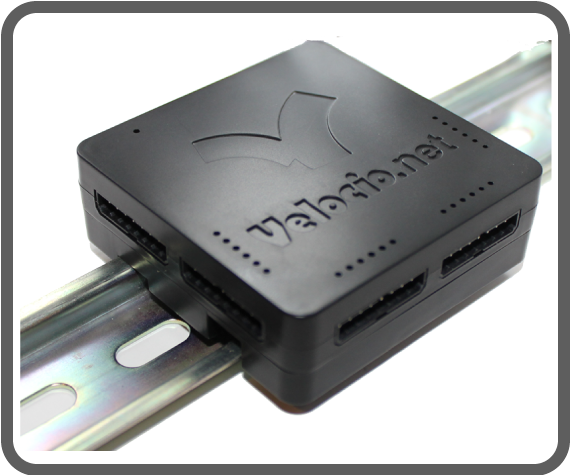
\includegraphics[width=.9\linewidth]{./img/Ace11.png}
\end{center}
\end{frame}

\begin{frame}[label={sec:org97a0077}]{Cyberphysical Target: The ACE 11 PLC}
\begin{itemize}
\item Small, inexpensive programmable logic controller
\item Programmable by Modbus over USB
\item Microcontroller is a TI 32-bit ARM Cortex-M4F (TM4C123H6PM)
\item Runs in Thumb-2 mode
\item 256kB flash memory, 2kB EEPROM, 32kB SRAM
\item 16-bit SIMD vector processing unit
\item multiple timers
\item single-precision floating-point unit
\end{itemize}
\end{frame}

\begin{frame}[label={sec:org7d41a0c}]{Domain}
In the initial phase of our research, we are restricting our focus to \alert{Boolean functions}, as implemented on the ACE 11 programmable logic controller.
\end{frame}

\begin{frame}[label={sec:org97f646b}]{Boolean Symbolic Expressions as Genotypes}
We are searching for human-readable, formal specifications of Boolean functions, in the form of symbolic expression trees.

\begin{center}
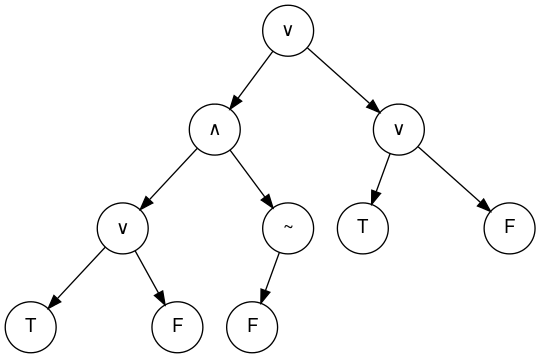
\includegraphics[width=.9\linewidth]{./img/boolean_sexp.png}
\end{center}

So we initialize a population of random Boolean expressions.
\end{frame}

\begin{frame}[label={sec:orgba15751}]{Symbolic Regression through Genetic Programming}
Our methodological starting point will be to build a genetic programming (GP) system for symbolic regression.

\begin{itemize}
\item initialize a random population of function specifications (\alert{genotypes})
\item embed this population in a spatial or ``\alert{geographical}'' structure
\item iteratively evaluate random neighbourhoods of genotypes, in \alert{tournaments}
\item assign \alert{fitness} relative to how well a genotype's evaluation fits the available datapoints
\item cull the least fit of each batch
\item reproduce the most fit, through such \alert{genetic operators} as crossover and mutation
\end{itemize}
\end{frame}

\begin{frame}[label={sec:org5dd13c3}]{An Alternative to Tournament Selection: Lexicase Selection}
Here, we are dealing with what Lee Spector and Thomas Helmuth have called an ``uncompromising problem'',

\begin{quote}
a problem for which it is not acceptable for a solution to perform sub-optimally on any one test case in exchange for good performance on others.
\end{quote}

Helmuth and Spector have shown that for many such problems, their technique of \alert{lexicase selection} outperforms \alert{tournament selection}.
\end{frame}

\begin{frame}[label={sec:org8b6ee2a},fragile]{Lexicase Selection}
 \begin{verbatim}
1) Initialize:
   a) Set CANDIDATES to be the entire population.
   b) Set CASES to be a list of all the test cases in
   random order.

2) Loop:
   a) Set CANDIDATES to be the subset of the current
   CANDIDATES that have exactly the best performance
   of any individual currently in CANDIDATES for the
   first case in CASES.
   b) If CANIDATES contains just a single individual,
   then return it.
   c) If CASES contains just a single test case then
   return a randomly selected individual from CANDIDATES.
   d) Otherwise, remove the first test case from CASES
   and go to Loop.
\end{verbatim}
\end{frame}



\begin{frame}[label={sec:orga905f54}]{Opening the Black Box}
\begin{itemize}
\item So far, we have been treating the problem of recovering symbolic mathematical specifications from implementations as a \alert{black box} problem, where all we have at our disposal is a set of the black box's inputs and outputs.
\item But in doing so we leave a tremendous amount of information on the table.
\item How can we put this additional information to use?
\end{itemize}
\end{frame}


\begin{frame}[label={sec:orgd93e005}]{Constraint-Driven Genetic Programming (CDGP)}
\begin{itemize}
\item Technique developed by Iwo Błądek and Kryzysztof Krawiec (see their 2019 paper, ``Solving Symbolic Regression Problems with Formal Constraints'').
\item Begin by creating an initial set of tests \alert{T} that any solution must pass: generate a random set of inputs for \emph{f} and collecting the outputs.
\item Establish a set of formal properties \alert{C} that \emph{f} is either certain or highly likely to satisfy.
\item Generate an initial population of symbolic expressions, \alert{P}, each of which expresses a Boolean function of \emph{n} variables.
\end{itemize}
\end{frame}

\begin{frame}[label={sec:org0c2f115}]{Constraint-Driven Genetic Programming (cont.)}
\begin{itemize}
\item Perform tournament or lexicase selection on \alert{P}, to select a mating pair.
\item Enlist an SMT solver (Z3, for instance) to attempt to generate an input that, when passed to our selected candidates, violates one or more of the constraints in \alert{C}.
\item If such an input can be generated, it will be considered a counterexample to our candidate solutions, and will be fed to \emph{f} in order to generate a new datapoint, which will be appended to \alert{T}.
\end{itemize}
\end{frame}

\begin{frame}[label={sec:org130444a}]{Constraint-Driven Genetic Programming (cont.)}
\begin{itemize}
\item If, for some candidate \alert{x}, no such counterexample can be found, and \emph{all} of the tests in \alert{T} have been passed without any errors, then we are finished: the symbolic expression \alert{x} can be taken as a probable specification for the function implemented in \emph{f}.
\item So long as this is not the case, we apply one or more genetic operators (crossover, mutation) to the winning candidates, and insert the resulting offspring into \alert{P}, replacing whichever individuals were first eliminated by the lexicase selection process.
\end{itemize}
\end{frame}

\begin{frame}[label={sec:orgeff130f}]{Constraint-Driven Genetic Programming (cont.)}
\begin{itemize}
\item We repeat the process until a solution is found.
\item Once a solution has been found, we test it against a fresh battery of input/output pairs (datapoints) generated by \emph{f}, to better gauge the accuracy of our search. In any inaccuracies are detected, the discriminating tests are appended to \alert{T}, and we resume the search. If not, we consider the search complete.
\end{itemize}

\begin{block}{But where do our constraining properties come from?}
\end{block}
\end{frame}

\begin{frame}[label={sec:orgf9313d4}]{Probabilistic Property Testing}
\begin{itemize}
\item Since we have at our disposal not merely a subset of the target function's graph, but the implementation itself, we can employ this implementation as an ``oracle''. We can feed it any input we like and record its output.

\item This gives us all we need to avail ourselves of the mathematical theory of \emph{probabilistic property testing}.

\item This is a technique for determining whether or not a function \emph{f} satisfies, with high probability, a given property \emph{P}, on the basis of observing the behaviour of \(f(x)\) for a relatively small number of inputs \(x\) --- or else if \emph{f} is ``far'' from every function that satisfies \emph{P}.

\item We plan on developing a Julia library that can be used to perform PPT on arbitrary black-boxed functions, or oracles.
\end{itemize}
\end{frame}


\begin{frame}[label={sec:org80327d4}]{Static Program Analysis}
\begin{itemize}
\item A wealth of information about the structure of \emph{f} can be obtained through traditional static binary analysis.
\item By constructing and inspecting the \emph{data-flow graph} (DFG) for \emph{f}, for instance, we are able to determine which parameters contribute to value of \emph{f}.
\item An inspection of \emph{f}'s \emph{control-flow graph} (CFG) may allow us to assess \emph{f}'s worst-case computational complexity, relative to input.
\end{itemize}
\end{frame}

\begin{frame}[label={sec:org624c78c}]{Summary}
\begin{itemize}
\item Our approach to formula recovery goes from \alert{outside} to \alert{inside}, rather than the reverse.
\item This provides a degree of robustness against code obfuscation, since the \alert{execution behaviour} of the implementation is our primary source of information.
\item We begin with a black box, and then progressively \alert{constrain} the search for symbolic specification by bringing constraints into play.
\item These constraints may come from \alert{heterogeneous} sources: probabilistic property testing, static analysis, and perhaps others can be added as we go.
\end{itemize}
\end{frame}
\end{document}
